


In a further analysis, we find that, for homeowners who buy-and-sell in the short run, improved homes have higher returns than unimproved homes. This is perhaps because homeowners who buy-and-sell in the short run tend to have investment motive right at the time of purchase and therefore their choices and decisions are more guided by making economic gains. On the other hand, homeowners who buy-and-sell over longer periods of time are less likely to have investment motive at the time of purchase, but rather, consume and enjoy the housing services and other social benefits at the price of lower returns.

Over the last 26 years, for period 1990 - 2016, expenditure on home improvement, new dwelling and alteration and additions, in Australia, has increased nearly four folds , similar patterns have been observed around the globe (insert reference). 

however there exists an increasing pattern in the amount individuals further invest in housing in the form of home improvement. Over the last 26 years, home improvement expenditures have increased, both in real terms and as a component of the total residential investment . 



The 'Other residential' category is a building other than houses primarily used for long-term residential purposes and which contains (or has attached to it) more than one dwelling unit for e.g. it includes blocks of flats, home units, attached townhouses, semi-detached houses, duplexes\footnote{Duplexes are considered in the 'Other residential buildings' and Australian Bureau of Statistics does not provide a separate development cost values}. The expenditure on 'other residential' buildings have accelerated in recent years which is evident in the large number of developments of high rise building in the country. In this paper, we focus only on the home improvements for 'Houses' as the building type. 


For many households, buying a house is the largest financial decision they will make in their lifetime and they spend a sizeable portion of their income on their home. there exists an increasing pattern in the amount individuals further invest in housing in the form of home improvement.




\begin{figure}[!ht]
\centering
  %\subfloat[Total Value of Building Approvals Trend]{%
  %    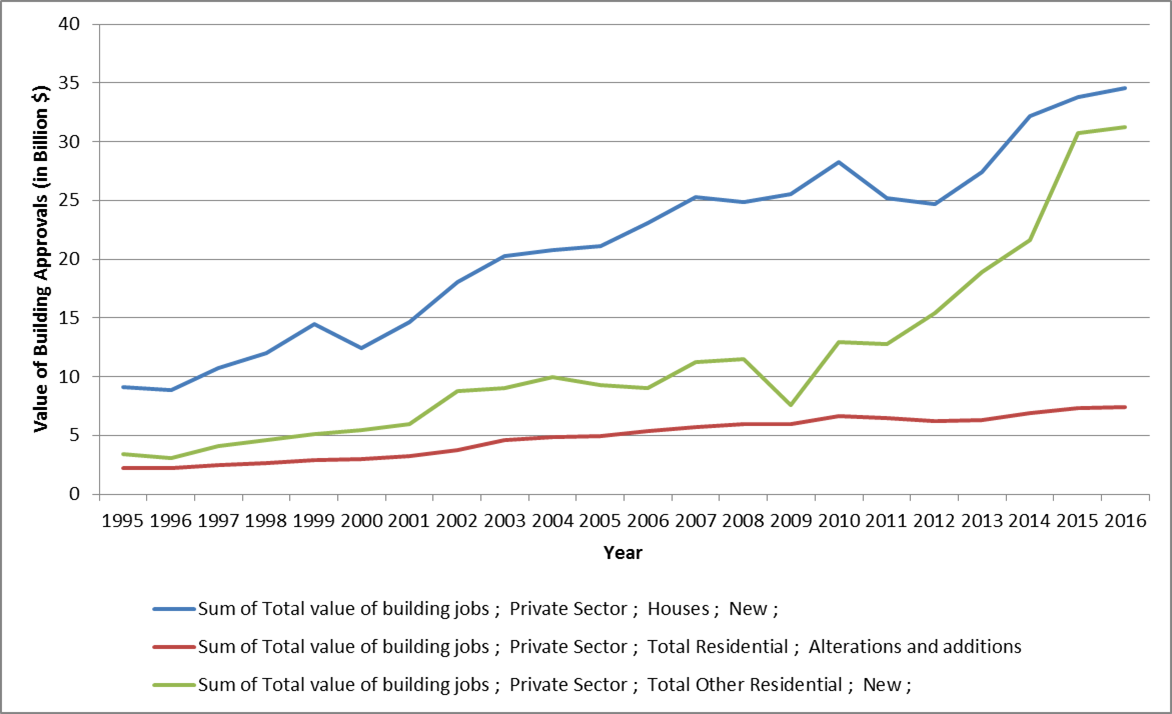
\includegraphics[width=0.75\textwidth]{Figures/Value_building_approvals.png}}\    
  \subfloat[Total Value of Building Approvals]{%
    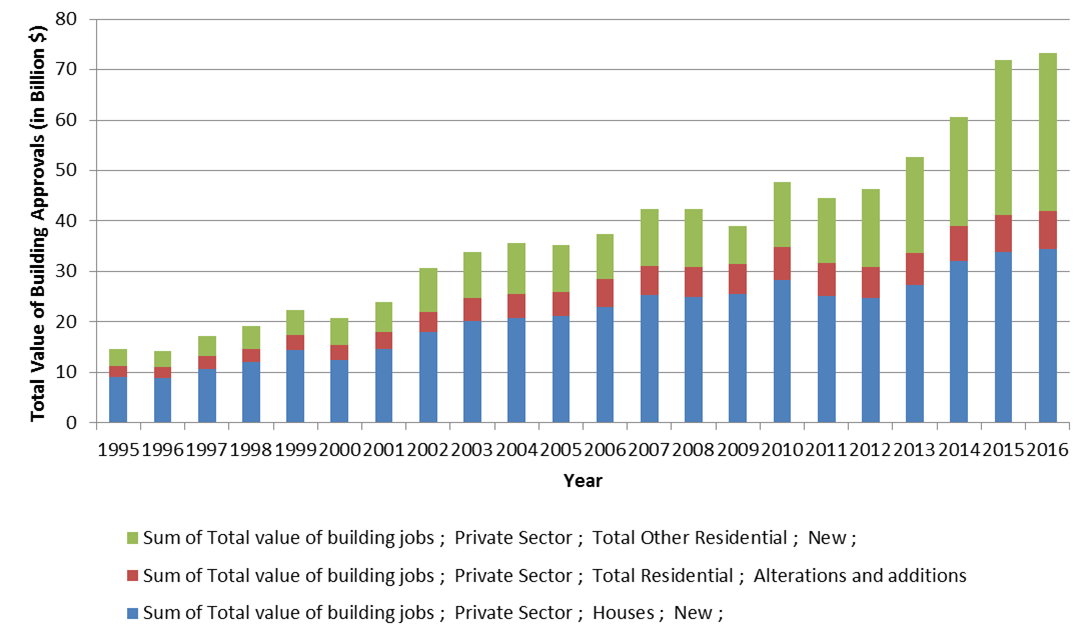
\includegraphics[width=0.75\textwidth]{Figures/ABS_Building_Approvals.png}}\  
 \caption{\small{Panels (A) and (B) show total value of Building Approvals trend and relative percentages}}
\label{fig:Total_Value_of_Building_Approvals}
Source: \scriptsize{Australian Bureau of Statistics}
\end{figure}





\citet{boehm1986improvement} studies the determinants of home improvement expenditures using a data sample created from surveys. The author starts with a production function $Q = Q(K0,M)$ that satisfies the second order conditions i.e. it is assumed to be twice differential with first derivative as positive i.e. for every unit increase in the home improvement input there is a positive gain from housing improvement and second derivative as negative i.e. the marginal gain from every additional home improvement input decreases. The author then derives a marginal benefit function of home improvements. 



The marginal benefit curve is negatively sloped under the assumptions that the marginal valuation of housing services declines with the quantity of housing services consumed and that the marginal product of home improvement input declines as home improvement increases. This is also in line with our empirical finding in this paper.  \citet{boehm1986improvement} 

The marginal product of home improvement input indicates the increase in housing services obtained from an additional dollar of expenditure. The author suggest that this will vary with the length of time the home improvement services are consumed and therefore we can include the age of home improvement in our model.

The marginal product of home improvement input indicates the increase in housing services obtained from an additional dollar of expenditure. The author suggest that this will vary with the length of time the home improvement services are consumed and therefore we can include the age of home improvement in our model.

The author says that the age of home improvement is ambiguous in terms of predicting the home improvement expenditures. An increase in age lowers the present value of change in resale value which reduces the investment incentive for improvement. However on other hand, lengthening the stream of future consumption benefits obtained from home improvement, an increase in the age stimulates the consumption motive for improvement.

However the author does not account for the fact that increasing the length of time owners stay in their homes also increases the house price due to appreciation and therefore increases the present value. We use the age of home improvement in explaining the returns from home improvement and find it to be significant and negatively sloped. In this paper we do not analyse the returns in terms of present values but instead we use the future value at the time of resale by indexing the previous sales price using a SSD (Statistical Sub Division) level hedonic index.

\citet{boehm1986improvement} also find that in addition to some other variables, the rate of property taxation had an insignificant effect on the amount household are willing to spend on home improvements.

To motivate empirical work, we consider a model similar to that of \citet{boehm1986improvement}.


This rationalizes our use of CPI as a means for inflating the cost if they were to be spent at the time of current sale. So if the homeowners were to spend money tomorrow they would have to compensate for the lost buying power due to inflation. They also test these hypothesis using an empirical data set.


We use the difference between the actual sale price and the expected sale price derived from the previous sale as the dependent variable with home expenditures as the independent variable. We use the length of time home owners spend in their home before a resale to account for the utility they derive from the consumption.


According to \citet{potepan1989interest}, there are technological constraints, for example, the presence of existing housing constraints the home improvement by impeding the application of certain construction techniques common in new housing production. For relatively modest increases in housing demand, this technological difference is probably negligible. For sizable increases, this technological constraint results in higher average costs in home improvement. This probably is one of the reasons which explains why, in our results we find that the marginal return on new house is higher than all other DA types. Author also says that while new housing is produced under constant returns to scale, improved housing is produced under decreasing returns to scale which is also true in our model.



The estimated coefficient have expected signs. The coefficient on the market returns The returns reduce as the age of the house increases. 


While the fixed-effects specifications are estimated on small samples and accordingly have less statistical power than the main analysis, the estimation results generally confirm
the main findings.


\subsection{Institutional setting}
Once the application is received, the council reviews the development plan and if it satisfies the requirements, the development approval is granted to the homeowners. This is the date when building approval is received that we use in our model as the date of improvement.

The value of additional housing acquired through home improvement is unobserved until the property is sold. When the property is sold the value of additional housing will be implicit in the sale price. Therefore in our analysis we consider only the repeat sales records with a development work carried out between those repeat sales. 




below the model....

According to \citet{combes2016production} any profits that are generated are dissipated into the land. Therefore any growth in the value over time that an individual attaches to the housing service is dissipated into the land value. Hence, the value of the housing service remains the same but land appreciates. We assume that the house prices follow a log-normal distribution. So at T = 0, the expected value of house is given by,

$$V_{0}=L_{-1} e^{rt_1} + C_{-1} e^{-dt_1} + H_{-1} e^{st_1}$$ where $r$ is the continuously compounding land appreciation rate due to the supply and demand of land. $d$ is the continuously compounding depreciation rate of the building and $s$ is the appreciation of housing service value. . Therefore using the house price index we calculate the expected house price before the completion of DA. 




We assume that the production function for housing uses existing housing stock $H_0$ and capital $K$ as primary inputs. $H_0$ comprises of all the existing housing elements, including land. $H_0$ is fixed and the only variable is capital.

$$ log(I_0) = Q(H_0 , K) $$ Therefore, 

$$ log(P_{+1}-E(P_{+1})) = Q(H_0,K) + H - dt_2 $$

The difference between the contract price and the expected contract price is the premium that is paid for the housing value created through home improvements. For intuitive interpretation, the above model is estimated in dollar value using the repeat sales data.

House builders maximise profit when carrying out home improvement. They choose the level of capital investment in order to build additional housing services given the amount of land and other existing housing services..

The profit function can be given as $\pi = P_{+1} - E(P_{+1}) - r*DA cost$




data

%% Table generated by Excel2LaTeX from sheet 'Count Distribution'
\begin{table}[h]
  \centering
  \caption{Distribution of DAs by type and state (Individual DAs)}
 \resizebox{\columnwidth}{!}{
    \begin{tabular}{lrrrrrrr}
    \toprule
          & \multicolumn{7}{c}{State} \\
\cmidrule{2-8}    DA Type & \multicolumn{1}{c}{NSW} & \multicolumn{1}{c}{QLD} & \multicolumn{1}{c}{SA} & \multicolumn{1}{c}{TAS} & \multicolumn{1}{c}{VIC} & \multicolumn{1}{c}{WA} & \multicolumn{1}{c}{Total} \\
    \midrule
    Duplex &               663  &             -    &                 1  &              -    &               137  &                   -    &                 801  \\
    Extension \& Alteration &           5,355  &         945  &             928  &             78  &           3,884  &            1,763  &            12,953  \\
    Garages/Sheds \& Carports &               392  &         395  &             139  &             24  &               239  &                223  &              1,412  \\
    House/Single Dwelling &           2,040  &      1,346  &          1,017  &             20  &           3,723  &            4,127  &            12,273  \\
    Swimming Pool &           5,031  &      4,699  &          1,644  &             11  &           3,715  &            8,175  &            23,275  \\
    Verandahs \& Pergolas &           1,289  &      2,447  &          2,188  &           117  &           3,390  &            6,198  &            15,629  \\
    Total &         14,770  &      9,832  &          5,917  &           250  &         15,088  &          20,486  &            66,343  \\
    \bottomrule
    \end{tabular}%
    }
  \label{tab:dist_da_state_type}%
\end{table}%

%% Table generated by Excel2LaTeX from sheet 'Count Distribution'
\begin{table}[!ht]
  \centering
  \caption{Distribution of DAs by type and state (Between Repeat Sales)}
  \resizebox{\columnwidth}{!}{
    \begin{tabular}{lrrrrrrr}
    \toprule
          & \multicolumn{7}{c}{State} \\
\cmidrule{2-8}    DA Type & \multicolumn{1}{c}{NSW} & \multicolumn{1}{c}{QLD} & \multicolumn{1}{c}{SA} & \multicolumn{1}{c}{TAS} & \multicolumn{1}{c}{VIC} & \multicolumn{1}{c}{WA} & \multicolumn{1}{c}{Total} \\
    \midrule
    Duplex &               613  &       &                 1  &       &               122  &       &                 736  \\
    Extension/Alteration &           4,669  &           681  &             727  &             74  &           3,437  &            1,221  &            10,809  \\
    Garages/Sheds \& Carports &               302  &           307  &               98  &             23  &               194  &                151  &              1,075  \\
    House/Single Dwelling &           1,479  &           590  &             516  &             15  &           2,686  &                792  &              6,078  \\
    Swimming Pool &           4,007  &        3,701  &          1,248  &               9  &           2,703  &            5,052  &            16,720  \\
    Verandahs \& Pergolas &           1,097  &        2,053  &          1,737  &           109  &           2,795  &            4,274  &            12,065  \\
    Multiple DAs between repeat sale &           1,275  &        1,225  &             773  &             10  &           1,546  &            4,353  &              9,182  \\
    Total &         13,442  &        8,557  &          5,100  &           240  &         13,483  &          15,843  &            56,665  \\
    \bottomrule
    \end{tabular}%
    }
  \label{tab:dist_da_state_type_bet_rs}%
\end{table}%




%may be talk something on the distribution and statistics here..

%% Table generated by Excel2LaTeX from sheet 'Count Distribution'
\begin{table}[htbp]
  \centering
  \caption{Descriptive Statistics for DA cost\$ (Individual DAs)}
   \resizebox{\textwidth}{!}{
    \begin{tabular}{rccccccc}
    \toprule
          & \multicolumn{7}{c}{Mean} \\
          & \multicolumn{7}{c}{\textit{(Std. deviation)}} \\
          & \multicolumn{7}{c}{obs.} \\
\cmidrule{2-8}    \multicolumn{1}{l}{DA Type} & NSW   & QLD   & SA    & TAS   & VIC   & WA    & Total \\
    \midrule
    \multicolumn{1}{l}{Duplex} & 447,629 &       & 150,000 &       & 661,942 &       & 483,913 \\
          & \textit{(226,765)} &       & \textit{NA} &       & \textit{(251,448)} &       & \textit{(244,864)} \\
          & 663   &       & 1     &       & 137   &       & 801 \\
    \multicolumn{1}{l}{Extension/Alteration} & 97,723 & 51,646 & 73,483 & 69,865 & 121,306 & 104,825 & 100,495 \\
          & \textit{(102,928)} & \textit{(60,604)} & \textit{(64,770)} & \textit{(73,028)} & \textit{(134,600)} & \textit{(128,253)} & \textit{(114,087)} \\
          & 5,355 & 945   & 928   & 78    & 3,884 & 1,763 & 12,953 \\
    \multicolumn{1}{l}{Garages/Sheds \& Carports} & 16,163 & 12,754 & 9,868 & 13,289 & 12,683 & 12,944 & 13,443 \\
          & \textit{(11,131)} & \textit{(8,743)} & \textit{(5,582)} & \textit{(7,887)} & \textit{(11,440)} & \textit{(9,316)} & \textit{(9,953)} \\
          & 392   & 395   & 139   & 24    & 239   & 223   & 1,412 \\
    \multicolumn{1}{l}{House/Single Dwelling} & 264,278 & 256,952 & 203,651 & 194,498 & 335,801 & 268,957 & 281,607 \\
          & \textit{(190,231)} & \textit{(133,019)} & \textit{(108,906)} & \textit{(107,385)} & \textit{(241,836)} & \textit{(225,188)} & \textit{(212,876)} \\
          & 2,040 & 1,346 & 1,017 & 20    & 3,723 & 4,127 & 12,273 \\
    \multicolumn{1}{l}{Swimming Pool} & 23,990 & 24,219 & 23,012 & 29,818 & 34,956 & 19,940 & 24,298 \\
          & \textit{(18,986)} & \textit{(10,990)} & \textit{(15,023)} & \textit{(27,777)} & \textit{(25,079)} & \textit{(60,378)} & \textit{(39,041)} \\
          & 5,031 & 4,699 & 1,644 & 11    & 3,715 & 8,175 & 23,275 \\
    \multicolumn{1}{l}{Verandahs \& Pergolas} & 17,441 & 12,430 & 11,470 & 14,932 & 14,362 & 9,415 & 11,951 \\
          & \textit{(12,761)} & \textit{(10,399)} & \textit{(8,200)} & \textit{(16,759)} & \textit{(12,524)} & \textit{(6,873)} & \textit{(10,051)} \\
          & 1,289 & 2,447 & 2,188 & 117   & 3,390 & 6,198 & 15,629 \\
    \multicolumn{1}{l}{All DA} & 102,148 & 55,322 & 57,420 & 46,934 & 132,132 & 74,150 & 89,185 \\
          & \textit{(152,254)} & \textit{(97,066)} & \textit{(87,541)} & \textit{(72,206)} & \textit{(195,797)} & \textit{(152,664)} & \textit{(154,815)} \\
          & 14,770 & 9,832 & 5,917 & 250   & 15,088 & 20,486 & 66,343 \\
    \bottomrule
    \end{tabular}%
    }
  \label{tab:DA_statistics}%
\end{table}%

%% Table generated by Excel2LaTeX from sheet 'Sheet15'
\begin{table}[htbp]
  \centering
  \caption{\scriptsize{Descriptive Statistics for DA cost (constant \$ Q3-2016) (Individual DAs)}}
   \resizebox{\textwidth}{!}{%
   \begin{tabular}{rrrrrrrr}
    \toprule
          & \multicolumn{7}{c}{Mean} \\
          & \multicolumn{7}{c}{\textit{(Std. deviation)}} \\
        & \multicolumn{7}{c}{obs.} \\
    \midrule
    \multicolumn{1}{l}{DA Type} & \multicolumn{1}{c}{NSW} & \multicolumn{1}{c}{QLD} & \multicolumn{1}{c}{SA} & \multicolumn{1}{c}{TAS} & \multicolumn{1}{c}{VIC} & \multicolumn{1}{c}{WA} & \multicolumn{1}{c}{All states} \\
    \midrule
    \multicolumn{1}{l}{Duplex} &       493,845  &       &       172,374  &       &       743,670  &       &        536,173  \\
          & \textit{  (237,953) } &       & \multicolumn{1}{c}{\textit{ NA }} &       & \textit{   (288,546) } &       & \textit{   (264,635) } \\
          & 663   &       & 1     &       & 137   &       & 801 \\
    \multicolumn{1}{l}{Extension/Alteration} &       113,008  &         62,017  &         88,154  &         82,577  &       145,152  &       127,612  &        118,950  \\
          & \textit{  (116,461) } & \textit{     (74,618) } & \textit{     (77,798) } & \textit{     (86,125) } & \textit{   (159,452) } & \textit{   (152,510) } & \textit{   (133,490) } \\
          & 5,355 & 945   & 928   & 78    & 3,884 & 1,763 & 12,953 \\
    \multicolumn{1}{l}{Garages/Sheds \& Carports} &         18,136  &         14,937  &         11,014  &         15,191  &         14,465  &         14,844  &          15,349  \\
          & \textit{     (12,836) } & \textit{     (10,193) } & \textit{       (6,068) } & \textit{       (8,569) } & \textit{     (13,090) } & \textit{     (10,782) } & \textit{      (11,441) } \\
          & 392   & 395   & 139   & 24    & 239   & 223   & 1,412 \\  
    \multicolumn{1}{l}{House/Single Dwelling} &       308,261  &       310,021  &       236,243  &       222,575  &       387,710  &       321,213  &        330,803  \\
          & \textit{  (218,475) } & \textit{   (163,402) } & \textit{   (126,252) } & \textit{   (119,269) } & \textit{   (285,058) } & \textit{   (270,348) } & \textit{   (251,638) } \\
            & 2,040 & 1,346 & 1,017 & 20    & 3,723 & 4,127 & 12,273 \\  
    \multicolumn{1}{l}{Swimming Pool} &         29,144  &         29,666  &         27,978  &         37,589  &         41,930  &         24,458  &          29,566  \\
          & \textit{     (22,538) } & \textit{     (13,192) } & \textit{     (18,322) } & \textit{     (32,880) } & \textit{     (31,423) } & \textit{     (78,656) } & \textit{      (50,332) } \\
         & 5,031 & 4,699 & 1,644 & 11    & 3,715 & 8,175 & 23,275 \\
    \multicolumn{1}{l}{Verandahs \& Pergolas} &         20,377  &         15,308  &         12,892  &         18,427  &         16,719  &         10,816  &          13,936  \\
          & \textit{     (15,193) } & \textit{     (12,979) } & \textit{       (9,041) } & \textit{     (21,402) } & \textit{     (14,689) } & \textit{       (8,019) } & \textit{      (11,920) } \\
          & 1,289 & 2,447 & 2,188 & 117   & 3,390 & 6,198 & 15,629 \\
    \multicolumn{1}{l}{All DA Types} &       117,903  &         66,991  &         67,259  &         55,306  &       154,096  &         88,886  &        104,876  \\
          & \textit{  (171,402) } & \textit{   (117,667) } & \textit{   (101,910) } & \textit{     (83,253) } & \textit{   (227,875) } & \textit{   (183,779) } & \textit{   (181,101) } \\
           & 14,770 & 9,832 & 5,917 & 250   & 15,088 & 20,486 & 66,343 \\
    \bottomrule
    \end{tabular}%
    }%
  \label{tab:DA_statistics_constant_dollar}%
\end{table}%


%% Table generated by Excel2LaTeX from sheet 'Count Distribution'
\begin{table}[!htbp]
  \centering
  \caption{Descriptive Statistics for DA cost \$ (Repeat Sales Level)}
   \resizebox{0.9\textwidth}{!}{%
    \begin{tabular}{rccccccc}
    \toprule
          & \multicolumn{7}{c}{Mean} \\
          & \multicolumn{7}{c}{\textit{(Std. deviation)}} \\
          & \multicolumn{7}{c}{obs.} \\
\cmidrule{2-8}    \multicolumn{1}{l}{DA Type} & NSW   & QLD   & SA    & TAS   & VIC   & WA    & Total \\
    \midrule
    \multicolumn{1}{l}{Duplex} & 463,211 &       & 160,399 &       & 703,367 &       & 502,608 \\
          & \textit{(227,379)} &       & \textit{NA} &       & \textit{(255,706)} &       & \textit{(248,912)} \\
          & 613   &       & 1     &       & 122   &       & 736 \\
    \multicolumn{1}{l}{Extension/Alteration} & 102,411 & 61,375 & 78,806 & 77,054 & 128,392 & 120,419 & 108,360 \\
          & \textit{(104,633)} & \textit{(69,442)} & \textit{(65,224)} & \textit{(80,168)} & \textit{(135,316)} & \textit{(131,975)} & \textit{(116,241)} \\
          & 4669  & 681   & 727   & 74    & 3437  & 1221  & 10809 \\
    \multicolumn{1}{l}{Garages/Sheds \& Carports} & 16,410 & 13,943 & 10,700 & 14,561 & 13,557 & 13,883 & 14,275 \\
          & \textit{(11,755)} & \textit{(9,767)} & \textit{(6,243)} & \textit{(8,373)} & \textit{(11,830)} & \textit{(8,250)} & \textit{(10,398)} \\
          & 302   & 307   & 98    & 23    & 194   & 151   & 1075 \\
    \multicolumn{1}{l}{House/Single Dwelling} & 275,079 & 267,882 & 224,155 & 229,962 & 353,989 & 369,398 & 317,108 \\
          & \textit{(180,358)} & \textit{(112,792)} & \textit{(121,085)} & \textit{(127,106)} & \textit{(256,953)} & \textit{(299,785)} & \textit{(231,665)} \\
          & 1479  & 590   & 516   & 15    & 2686  & 792   & 6078 \\
    \multicolumn{1}{l}{Multiple\_DA} & 267,116 & 229,389 & 195,669 & 143,222 & 358,661 & 260,254 & 268,093 \\
          & \textit{(259,750)} & \textit{(201,570)} & \textit{(137,150)} & \textit{(102,347)} & \textit{(290,627)} & \textit{(246,255)} & \textit{(247,789)} \\
          & 1275  & 1225  & 773   & 10    & 1546  & 4353  & 9182 \\
    \multicolumn{1}{l}{Swimming Pool} & 25,874 & 26,850 & 25,038 & 32,519 & 38,135 & 22,249 & 26,918 \\
          & \textit{(15,398)} & \textit{(12,147)} & \textit{(17,840)} & \textit{(30,363)} & \textit{(30,718)} & \textit{(97,026)} & \textit{(56,015)} \\
          & 4007  & 3701  & 1248  & 9     & 2703  & 5052  & 16720 \\
    \multicolumn{1}{l}{Verandahs \& Pergolas} & 18,836 & 13,777 & 12,187 & 16,705 & 15,539 & 10,290 & 13,207 \\
          & \textit{(13,719)} & \textit{(11,753)} & \textit{(8,571)} & \textit{(19,713)} & \textit{(13,673)} & \textit{(7,477)} & \textit{(11,190)} \\
          & 1097  & 2053  & 1737  & 109   & 2795  & 4274  & 12065 \\
    \multicolumn{1}{l}{All Das} & 121,918 & 71,612 & 74,085 & 54,300 & 161,799 & 109,257 & 115,679 \\
          & \textit{(173,523)} & \textit{(123,245)} & \textit{(107,396)} & \textit{(82,213)} & \textit{(225,544)} & \textit{(200,764)} & \textit{(186,725)} \\
          & 13,442 & 8,557 & 5,100 & 240   & 13,483 & 15,843 & 56,665 \\
    \bottomrule
    \end{tabular}%
    }
  \label{tab:DA_stats_rs_level}%
\end{table}%

%% Table generated by Excel2LaTeX from sheet 'Count Distribution'
\begin{table}[!htbp]
  \centering
  \caption{Descriptive Statistics DA cost (constant\$ Q3-2016) (Repeat Sales)}
     \resizebox{0.9\textwidth}{!}{%
    \begin{tabular}{rccccccc}
    \toprule
          & \multicolumn{7}{c}{Mean} \\
          & \multicolumn{7}{c}{\textit{(Std. deviation)}} \\
          & \multicolumn{7}{c}{obs.} \\
\cmidrule{2-8}    \multicolumn{1}{l}{DA Type} & NSW   & QLD   & SA    & TAS   & VIC   & WA    & Total \\
    \midrule
    \multicolumn{1}{l}{Duplex} & 491,588 &       & 172,374 &       & 760,411 &       & 535,715 \\
          & \textit{(233,731)} &       & \textit{NA} &       & \textit{(278,275)} &       & \textit{(261,573)} \\
          & 613   &       & 1     &       & 122   &       & 736 \\
    \multicolumn{1}{l}{Extension/Alteration} & 108,680 & 65,979 & 85,029 & 82,035 & 138,954 & 130,004 & 116,252 \\
          & \textit{(109,639)} & \textit{(74,837)} & \textit{(69,375)} & \textit{(84,990)} & \textit{(145,312)} & \textit{(140,560)} & \textit{(123,702)} \\
          & 4669  & 681   & 727   & 74    & 3437  & 1221  & 10809 \\
    \multicolumn{1}{l}{Garages/Sheds \& Carports} & 17,179 & 14,935 & 11,061 & 15,296 & 14,279 & 14,528 & 15,044 \\
          & \textit{(12,799)} & \textit{(10,527)} & \textit{(6,329)} & \textit{(8,745)} & \textit{(12,468)} & \textit{(8,678)} & \textit{(11,135)} \\
          & 302   & 307   & 98    & 23    & 194   & 151   & 1075 \\
    \multicolumn{1}{l}{House/Single Dwelling} & 294,501 & 287,908 & 240,499 & 239,705 & 379,036 & 397,607 & 339,934 \\
          & \textit{(189,370)} & \textit{(116,243)} & \textit{(128,628)} & \textit{(128,905)} & \textit{(285,371)} & \textit{(324,503)} & \textit{(252,781)} \\
          & 1479  & 590   & 516   & 15    & 2686  & 792   & 6078 \\
    \multicolumn{1}{l}{Multiple\_DA} & 283,189 & 249,059 & 207,759 & 153,836 & 381,123 & 279,387 & 286,831 \\
          & \textit{(274,160)} & \textit{(215,857)} & \textit{(145,586)} & \textit{(104,467)} & \textit{(308,827)} & \textit{(259,608)} & \textit{(262,094)} \\
          & 1275  & 1225  & 773   & 10    & 1546  & 4353  & 9182 \\
    \multicolumn{1}{l}{Swimming Pool} & 27,886 & 29,250 & 27,049 & 35,975 & 40,972 & 24,318 & 29,168 \\
          & \textit{(16,436)} & \textit{(13,217)} & \textit{(18,550)} & \textit{(35,307)} & \textit{(32,921)} & \textit{(99,391)} & \textit{(57,616)} \\
          & 4007  & 3701  & 1248  & 9     & 2703  & 5052  & 16720 \\
    \multicolumn{1}{l}{Verandahs \& Pergolas} & 20,141 & 15,320 & 12,798 & 18,388 & 16,626 & 10,911 & 14,164 \\
          & \textit{(14,947)} & \textit{(12,891)} & \textit{(8,962)} & \textit{(21,682)} & \textit{(14,453)} & \textit{(7,987)} & \textit{(12,015)} \\
          & 1097  & 2053  & 1737  & 109   & 2795  & 4274  & 12065 \\
    \multicolumn{1}{l}{All Das} & 129,774 & 77,619 & 79,168 & 57,852 & 173,377 & 117,496 & 123,981 \\
          & \textit{(183,129)} & \textit{(132,336)} & \textit{(114,365)} & \textit{(86,003)} & \textit{(243,426)} & \textit{(213,383)} & \textit{(199,400)} \\
          & 13,442 & 8,557 & 5,100 & 240   & 13,483 & 15,843 & 56,665 \\
    \bottomrule
    \end{tabular}%
    }
  \label{tab:DA_stats_rs_level_const_dollar}%
\end{table}%



%\floatbarrier

%This method of identifying confirmed developments was robust with one disadvantage that we had to exclude observations where the previous attributes were missing and we cannot confirm change in attributes\footnote{One flag for identifying confirmed developments, was the presence of the builder name. To test the validity of the builder name flag, we looked at the distribution of the builder types in our robust sample. Of the robust records, we found that only 36\% of records had builder names available and almost 60\% of records had no builder names and the remaining 5\% were owner builders. This suggested that the builder name flag could not be used as a valid indicator of confirmed developments}. 

%% Table generated by Excel2LaTeX from sheet 'Count Distribution'
\begin{table}[!ht]
    \centering 
   
    \label{tab:da_relative_time}%  
        \resizebox{0.8\textwidth}{!}{%
            \begin{threeparttable}
               \caption{Descriptive Statistics - Time of DA relative to sales \tnote{a}}  
                
                
                
                
                \begin{tabular}{lcc}
                    \toprule
                    Variable & Mean  & Std. deviation \\
                    \cmidrule{2-3}          & \multicolumn{2}{c}{(In years)} \\
                    \midrule
                    Time between sales & 7.39  & 4.47 \\
                    Time to DA & 3.99  & 2.58 \\
                    Time to subsequent sale post DA & 3.40  & 3.57 \\
                    \bottomrule
                \end{tabular}%
                
                
                
                
                
                \begin{tablenotes}
                     \small
                     \item[a] Table shows the mean and standard deviation, in years, of time between sales, time to DA and time to subsequent sale post DA.
                \end{tablenotes}
                
            \end{threeparttable}
        }%
    
\end{table}%

%\floatbarrier


After filtering the data for,   we have roughly 5.4m total homes with repeat sales and 1.6m homes have development approvals, nationwide. On combining these two data sets, we have a sample of 259,428 homes that have repeat sales and development approvals received between the repeat sales. 

Homes that have a repeat sale but no development approval (4.1m records) are candidates for the control sample of unimproved homes.


 The house prices are recorded in CoreLogic's database when the property is either listed, sold, valued or financed. 


In the identified sample of 259,428 records, there could be some homes that received development approvals but haven't gone ahead with their development. Based on the available data, there is no definitive way to identify all the properties that have indeed improved their homes. It is important to distinguish between properties that have obtained building approvals but haven't gone ahead with the construction and those that have, since, if the property has not gone ahead with their development then we would have accounted for the improvement cost, however, the value of that improvement would be implicitly excluded from the contract price and therefore we would underestimate the returns and cause a downward bias.




While the main analysis relies on simple linear models estimated with least squares, we also examine a variety of functional forms and estimation techniques to demonstrate that the main findings are not an artifact of the least squares estimation within a non normal distribution. Least squares estimates can also be heavily be influenced by outlying observations, particularly in smaller samples. To prevent outlying observations from distorting the inferences from the regression analysis, we use a robust linear model estimation or winsorize the home improvement and house prices to $97.5^th$ percentile in small subsets.



however,  the  improved  homes  also  incur  a  cost  at  timet=  0  and  we  need  to account for that as well.  At time of DA the, the expectred price plus the cost of DAcan also be thought of as a notional purchase price.  As there the home improvementvalue is created after point of DA, and any value created in the house price is soleyattributed to the market appreciation.  therefore we can excluded the appreciationin value from t = -1 to t = 0.  The expected value at the time of DA plus the costof DA is equal to the notional purhase price and we can compare the returns fromimrovement homes with unimprovemnt homes.  For unimproved homes, we take allobservation from March 2004 as we have DA data available from March 2004 andwe would be unsure whether unimproved homes prior 2004 have actually done a DAor not.  Therefore to eliminate the bias, we consider non da home data from March2004.  For DA homes we calculate the expected value of homes at the point of DAstarting from 2004 and this can be thought of a point of notional purchase13



The study highlights an important financial friction that has suppressed residential investments. the evidence developed in this paper show that the returns on improved homes are not higher than non DA but raher even worse on average.
At roughly .... per year home imprvement spending nearly half as household savings and new construction




Housing is highly heterogeneous and land, an immobile factor whose price is often hard to observe, plays an important role in its production. these features call for specific estimation techniques, impose strong data constraints, and require careful attention to the sources of variation used for identification.

however, the improved homes also incur a cost at time $t = 0$ and we need to account for that as well. At time of DA the, the expectred price plus the cost of DA can also be thought of as a notional purchase price. As there the home improvement value is created after point of DA, and any value created in the house price is soley attributed to the market appreciation. therefore we can excluded the appreciation in value from t = -1 to t = 0. The expected value at the time of DA plus the cost of DA is equal to the notional purhase price and we can compare the returns from imrovement homes with unimprovemnt homes. For unimproved homes, we take all observation from March 2004 as we have DA data available from March 2004 and we would be unsure whether unimproved homes prior 2004 have actually done a DA or not. Therefore to eliminate the bias, we consider non da home data from March 2004. For DA homes we calculate the expected value of homes at the point of DA starting from 2004 and this can be thought of a point of notional purchase\footnote{There could be DAs prior 2004 in DA homes, in that case DAs cost would have have under estimated and the DA results would be even worse. We also run a after excluding the prior 2004 purchase for DA homes in the robustnes section}.




Firstly, the expected house price is the home equity at the time of DA approval that the homeowners have acquired due to market appreciation\footnote{One can argue that the home equity does not belong to the homeowners as there may be a loan on the property. however, assuming that the property prices have appreciated from the time between purchase and DA, the home equity is like holding an in-the-money option, so as long as there is no financial constraint and the value of the home equity is greater than the mortgage amount, the homeowners would continue to pay their mortgage and therefore, we can take that the home equity belongs to the homeowners as they can sell the property anytime, pay the loan and keep the profits.}. 




$$I_0 = b_0 + h_0$$

where, $b$ is the additional value of non-durable consumption and $h$ is the value of additional housing services created from the home improvement. This is the additional value that is produced from the home improvement that we want to measure. however this value is not observed at the point of DA.  



may be talk about omitted variable bias..
 belwo is the base model with endogeniety problem we find that hausamn test says that there is no endogeniety problme,,,, the area is a good instrument in our case.. but there is no endogeniety probelm..
 
 
 
 Since this paper seeks to explain the owner occupier based return on home improvement as opposed to rental renovations, the appropriate agent is not a profit maximizing landlord, but utility maximizing household. The landlord who buys the property with an investment motive
 
 
 
 
Finally, in improvement types like building a new house or building a new duplex, the homeowners demolish the existing building and develop a new house from scratch. However the existing building, after accounting for the depreciation, should have some residual building value, $B_0$ (the non-durable consumption) plus the housing service value, $H_0$ (the durable consumption). With the demolition of the old building, while the land value, $\alpha$ remains fixed, the non-durable value at the time of DA $B_0)$ is reduced to zero. This is the opportunity cost if the land were to be used for purposes other than residential. However, as the homeowner redevelops a house, the value of housing $H$ is regained and there is some additional housing value $H'$ created\footnote{Assuming that the homeowner builds a better home than the previous one.}. Therefore the opportunity cost of DA is only $B_0$. And cost is inseparable and observed implicitly in the Expected value of the home, calculated using the market index, at point of DA. Therefore to fully account for the costs, we need to calculate the expected purchase price at the time of DA\footnote{In case of other improvement types, the existing value of land, building and housing service remains intact, therefore there is no direct opportunity cost. When the home owner carries out development, the only cost is C, the cost of home improvement and the unobserved value created from home improvement is $H'$ which is indirectly observed in the resale price. Therefore there is no direct impact for to the other types of home improvements.}. 
 
 
 Now, the development occurs any time between a purchase and a resale, So at the time of DA, there is a cost incurred, which is observed at the time of building approval and there is a value produced at the time of development completion. Now, this value should equal to the building value (i.e. the cost of improvement) plus the value of additional housing produced by the improvement). The cost of construction is observed but the value of additional housing is unobserved at the time of DA. When the property sells subsequent DA, the additional value produced by DA will be implicitly observed in the resale price. This provides our identification strategy. 
 
 
 
 
 \subsection{Location Fixed Effect - Statistical Subdivision Level}

The main model controls for the geographical factors affecting the returns using the state fixed effects. However the house prices could vary significantly even within the state. For example, in NSW, house prices in capital city - Sydney could be considerably higher than prices in rest of the NSW. Since we model the returns, these variations in house prices should cancel out each other. Nonetheless, the geographical factor at lower level than state could still affect variations in the returns. Therefore we test the main results by controlling for the geographical factors at statistical subdivision (SSD) level.

Table \ref{tab:results_ssd} presents results for models 1 to 8 with SSD level location fixed effects. In models 7 and 8, we find that the results are consistent with the main results. The return, at aggregate level, for improved homes is 1.9\% and 2.4\% lower than unimproved homes respectively. 


When we look at by improvement types, the returns, as per models 1 to 6 are generally consistent with the main results. The coefficient for carports/garages/sheds is mostly insignificant. The returns for duplex is around 9\% higher than unimproved homes which is also consistent with the main results.

For extension/alterations, the returns were insignificant in the main results, however when we control at SSD level location fixed effects, the coefficient becomes significant around -1\%. For House/Single Dwelling, Multiple DAs, swimming pool and verandas/pergolas, the returns are consistent with the main results, around 11\%, 1.5\%, 0.7\% and 2.7\% lower than unimproved homes respectively. We also note that after controlling for location effects at SSD level, the $Mkt$ variable captures around 95\% of the variation in the returns as compared to 92\% with State level fixed effects.
 
 
 
 \subsection{SSD Index Validation}

To calculate the expected house price at the time of development approval, we use the statistical subdivision level house price index as provided by CoreLogic. Since all the properties have sales prices observed at least twice, we leverage the repeat sales information, to test whether the house price index is a good predictor of the market appreciation. We calculate the expected house price at time resale i.e at t = +1 and then calculate the percent prediction errors as $E(P_{+1})/P_{+1} - 1) * 100$. Finally, we plot the density, cumulative density function, QQ and PP plots of percent prediction errors as shown in the figure \ref{fig:Rplot_ssd_err_10}. 

\begin{figure}[!htb]
    \centering
     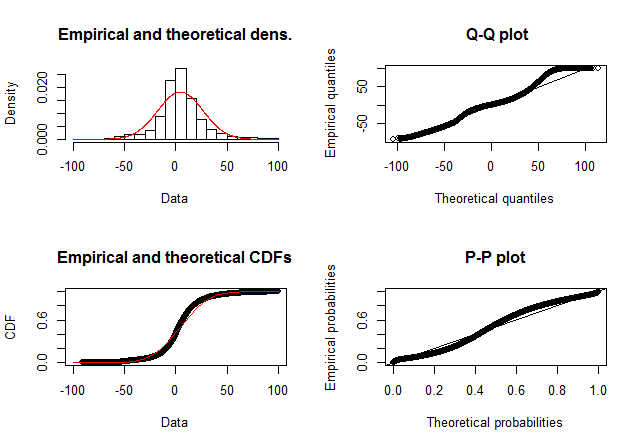
\includegraphics[width=\columnwidth]{Figures/Rplot_qqplot.png} \par
 \caption{House Price Index Prediction Error Distribution}
 \label{fig:Rplot_ssd_err_10}
\end{figure}

We see that the percent prediction error has a symmetric distribution around the mean and is heavily centered on zero. The bell shaped curve represents the normal distribution. The cumulative density fits the normal density. Also in the QQ plot and PP plot, the densities are similar to theoretical densities.


 
 
 
 notes from vito
 
 

Mention the one that comes close...and returns on maintenance spending

...literature...


There are several studies that have either modelled the demand for home improvement expenditures as a probability measure or the dollar value and there are other studies that have identified the determinants of home improvement expenditures. 




However, there is little work done in the literature that attempts to quantify the returns on home improvement. Some of the studies that come close mention here...

there are several studies done on housing maintenance....

several studies done on determinants of home improvement ....





\citet{gyourko2003urban} describes the role of construction costs in housing decline in America. Their main question in this paper is to study the sensitivity of investment to construction cost. They suggest that a rational investor would not invest in the housing if the home values are below replacement cost. There is often decay in the housing markets of declining areas. In their paper, they ask whether this process is endogenously demand driven or whether the supply side of the housing market plays some role. They find that housing prices are close to replacement cost in most areas. For houses in specific neighborhoods where the house prices are near construction costs, modest difference in replacement cost may be critical on the margin to determining whether a fundamental decay sets in or reinvestment occurs in the face of a negative demand shock. They say that the construction costs need not be exogenous to the decay process i.e. the construction costs may cause decay process which in turn may increase the construction cost and further induce the decay process. They suggest that if the construction cost were flexible downward in response to the negative demand shocks, then there need not even be a negative impact on housing investment. Their analysis finds that the construction costs are not very sensitive to construction levels. There is a substantial between city variations in the costs that cannot be account for with a standard, upward sloping supply schedule.



\citet{gyourko2004reinvestment} finds that demand for renovation services to be relatively price-inelastic. They also report that there is a substantial heterogeneity in the distribution of home values across different market areas. In places with high house value. A 1-percent drop in the construction cost would not change the fraction of homes with value above replacement costs. Land prices are so high in these areas that there are virtually no homes valued at less than 110 percent of the construction costs. They also confirmed that the relationship between renovation and home values is strongly linear. They confirmed this by introducing 20 dummies for each corresponding value quantile into regressions and they still could reject at the 5 or 10 percent levels. 



\citet{guthrie2010house} suggests that the new house prices are considerably above the direct construction costs. This premium can be attributed to the option value of delaying the development of marginal piece of land. Competition can reduce this option value but as long as there is heterogeneity in the land, the value cannot be reduced to zero. In the US data they find that this premium is economically significant.



Also \citet{boehm1986improvement} states that the investment return to home improvements depends on the price of housing services expected to prevail at the time the house is sold. However they do not estimate the relationship between investment return and the home improvement. The state that this price is positive function of the current neighborhood price of services and expected rate of house price appreciation and therefore uses other neighborhood quality variables such as crime rate in the area, quality of schools, roads, sidewalks etc. as explanatory variables in the empirical regression.   More specifically, the author suggests that the marginal benefit function represents the present value of the consumption benefits derived from additional unit of home improvement and the present value of change in resale value resulting from improvement which is the investment return on home improvements. However they do not attempt to measure the return on the home improvement. 



\citet{mendelsohn1977empirical} builds a theoretical model on home improvements and relate relates the amount of self labour invested in the home improvement as opposed to hired labour. The author suggests that homeowners work on their house until the rewards from that work are equal to the value of his leisure time. The reward of his work depends on his productivity, the market price of housing and the marginal utility of both housing and assets. The author also suggests that the marginal value of a dollar spent on housing improvements, assets or other goods should all be the same. 


However, from the homeowner’s perspective, there is a long standing question of the returns from home improvements. Are housing re-investments profitable? Do homeowners who improve their homes make better returns as compared to those who don't? Does the excess value attributed to the home improvement outweigh the costs? Also how do returns compare for homeowners who buy and sell with an investment motive as opposed to people who buy the property for self-living? These are some of the questions that we seek to answer.


\citet{helms2003understanding} models the determinants of urban housing renovation. The author suggests that in real world, households invariably take account of the asset value of their property when they make renovation decisions. However for simplicity they assume that household's return to their housing capital consist of only utility they derive from consuming the housing services that their investment provides. However, in this paper, we account for the asset value of the property.


Looking at development approvals directly, is notoriously difficult given that the improvements for different households occur at different points in time between a repeat sale. Also many household make a development application but never go ahead with the construction and therefore it becomes difficult to estimate the value of home improvement. When people buy and re-sell the property, they would make a return from the repeat sale. But if homeowners improve their homes in between the repeat sale, they would have also created some value from producing additional housing. The dynamics of both house price appreciation and the home improvement value also add to the challenge.



All these authors have explained the factors and how they affect the home improvement demand and the expenditures. However, there is no study that estimates the returns to home improvements. 


   also adds to the literature of choice modelling in the real options framework. Our paper provides 